%\addcontentsline{toc}{chapter}{Development Process}
\chapter{Design}

% You should concentrate on the more important aspects of the design. It is essential that an overview is presented before going into detail. As well as describing the design adopted it must also explain what other designs were considered and why they were rejected.

% The design should describe what you expected to do, and might also explain areas that you had to revise after some investigation.

% Typically, for an object-oriented design, the discussion will focus on the choice of objects and classes and the allocation of methods to classes. The use made of reusable components should be described and their source referenced. Particularly important decisions concerning data structures usually affect the architecture of a system and so should be described here.

% How much material you include on detailed design and implementation will depend very much on the nature of the project. It should not be padded out. Think about the significant aspects of your system. For example, describe the design of the user interface if it is a critical aspect of your system, or provide detail about methods and data structures that are not trivial. Do not spend time on long lists of trivial items and repetitive descriptions. If in doubt about what is appropriate, speak to your supervisor.
 
% You should also identify any support tools that you used. You should discuss your choice of implementation tools - programming language, compilers, database management system, program development environment, etc.

% Some example sub-sections may be as follows, but the specific sections are for you to define. 

\section{Overall Architecture}
The design of my application was evolutionary as I was developing it using XP in an agile way. This meant that each step had an initial design and was built upon every time a new feature was added, being refactored along the way. There were a number of prototypes made during the course of the project's development, and this chapter will discuss the design of the end product, and go into detail where the design may have been previously different.

The resulting application evolved into a web service, with a Model View Controller (MVC) framework and resources structured for maintainability. Following XPs guidelines, at each step of the way the applications design was made as such to be the simplest yet most maintainable it could be through refactoring, cutting down on duplicate code, structured logically and choosing smart data structures and Objects to represent aspects of the application and quality results.

\subsection{Choice of technologies}
At the beginning of the application, I felt that the application should be programmed in a language that would be able to be ported across multiple platforms for used by anybody who wished to use it. Additionally to this, I wanted to have ways of representing the components of my application as Objects and would need some way of presenting a UI to the user, even if my initial application would only output command line results, in order to follow the XP value of Simplicity (YAGNI - ``You Ain't Gonna Need It'', until you do).

For this reason, I selected to develop my application using Java to begin with as it filled the criteria of being Object Oriented and was portable through using the JVM on different operating systems. I resolved that I would select a UI package to present the report of my results once some of the core functionality had been implemented. I considered instead using Ruby or C++, but due to my familiarity with Java I believed it would be a better choice to stick with what I knew. At this point, I did not consider having the application as a web service, and so using Ruby with Rails was not something I had considered.

As the application developed and I started reading in files and outputting results from the GC Content process, I found that I was having a hard time finding a quickly usable GUI I could work with for Java to display the results in a way that I wanted. It was at this point I started considering a technology change to Ruby on Rails until Sion Griffiths, a peer of mine, suggested I could keep my application in Java and turn it into a web service using Spring Boot\cite{springboot}. This seemed like the perfect solution to my problem, allowing me to generate my charts and results using HTML5, JavaScript and HTML5 Canvas, along with JavaScript libraries such as  Plotly.js.

The conversion to Java Spring Boot was not a painful one, and only involved setting up a new Maven project and declaring it to run as a Spring Boot application in the pom.xml file, then copying over my previous code and structure into the new project, from there I could deploy the application as a web server using Tomcat and was back to my previous position of working out a UI. Thankfully, there is a package called Thymeleaf\cite{thymeleaf} that works with Spring Boot to allow access to Objects from within the Model of the Java code (placed there by the Controller) using the View dynamically as the View is generated through HTML templates and fragments.

\begin{figure}[H]
	\centering
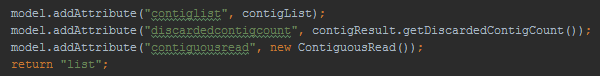
\includegraphics[width=1\textwidth]{images/addingtomodel}
\caption{Adding an object to the Model via the Controller to be accessed in the View. The View here is `list', which is a Thymeleaf template that will dynamically build the page using the data from the Model added here.}
\end{figure}

On top of using Thymeleaf for accessing data put into the Model, it has the additional benefit of using fragments that can be imported into different HTML templates. This design choice made it so I was able to cut down on writing duplicates of code. For example, I wrote the header and footer of the UI design in a Thymeleaf HTML fragment, and then on each page just need to call one line in order to import it into that page, rather than built the entire thing again. An extra benefit to this is that it allowed me to keep the HTML templates clean and easier to maintain by reducing their size and separating out different aspects of the UI. Having the header, footer and a number of forms in Thymeleaf HTML templates meant that these sections could be edited without impacting any page they are imported into.

\begin{figure}[H]
	\centering
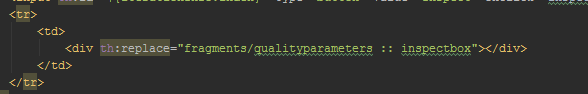
\includegraphics[width=1\textwidth]{images/thymeleafinsert1}
\caption{Including a thymeleaf fragment in a page. You can see how the call is made from one `th:replace' with the name of the html fragment file and then the fragment to be included from that file, in this case `inspectbox'.}
\end{figure}
\begin{figure}[H]
\centering
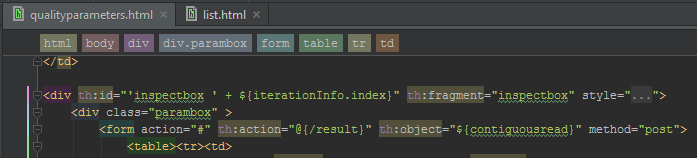
\includegraphics[width=1\textwidth]{images/thymeleafinsert2}
\caption{Including a thymeleaf fragment in a page. This is the declaration of the fragment being included in the previous figure, declared as such through `th:fragment'.}
\end{figure}

For the GUI itself, I elected to use Plotly for representing my GC content charts for the level of detail and control it gives a user over inspecting charts, large and small, that worked no matter what GC window size the user selected. For the ORF Locations frames charts I wrote my own code using JavaScript and displayed it with HTML5 Canvas, as it allowed me control over what should be shown depending what a user clicks upon and I could work with the data from the Model in ways I saw fit.

%=== Up to here

\subsection{MVC Framework}
As I was building an application with a GUI, the application was built using a Model View Controller framework design, separating out the components into their different types. This helped the separation of code and responsibilities. The class diagrams presented in this chapter are based on the final product design and based on a page per page view from the UI and what classes are used on the HTML request of that page.

\subsubsection{Model}
The Model was designed to contain the data and methods for processing a users input. This contains the data structures and objects for handling a users data as they traverse from page to page of the view. I designed the Model in a way that certain objects would be Bean objects (classes with getters and setters for their properties) that could be accessed by the View in the way that Thymeleaf required.

\begin{figure}[H]
\centering
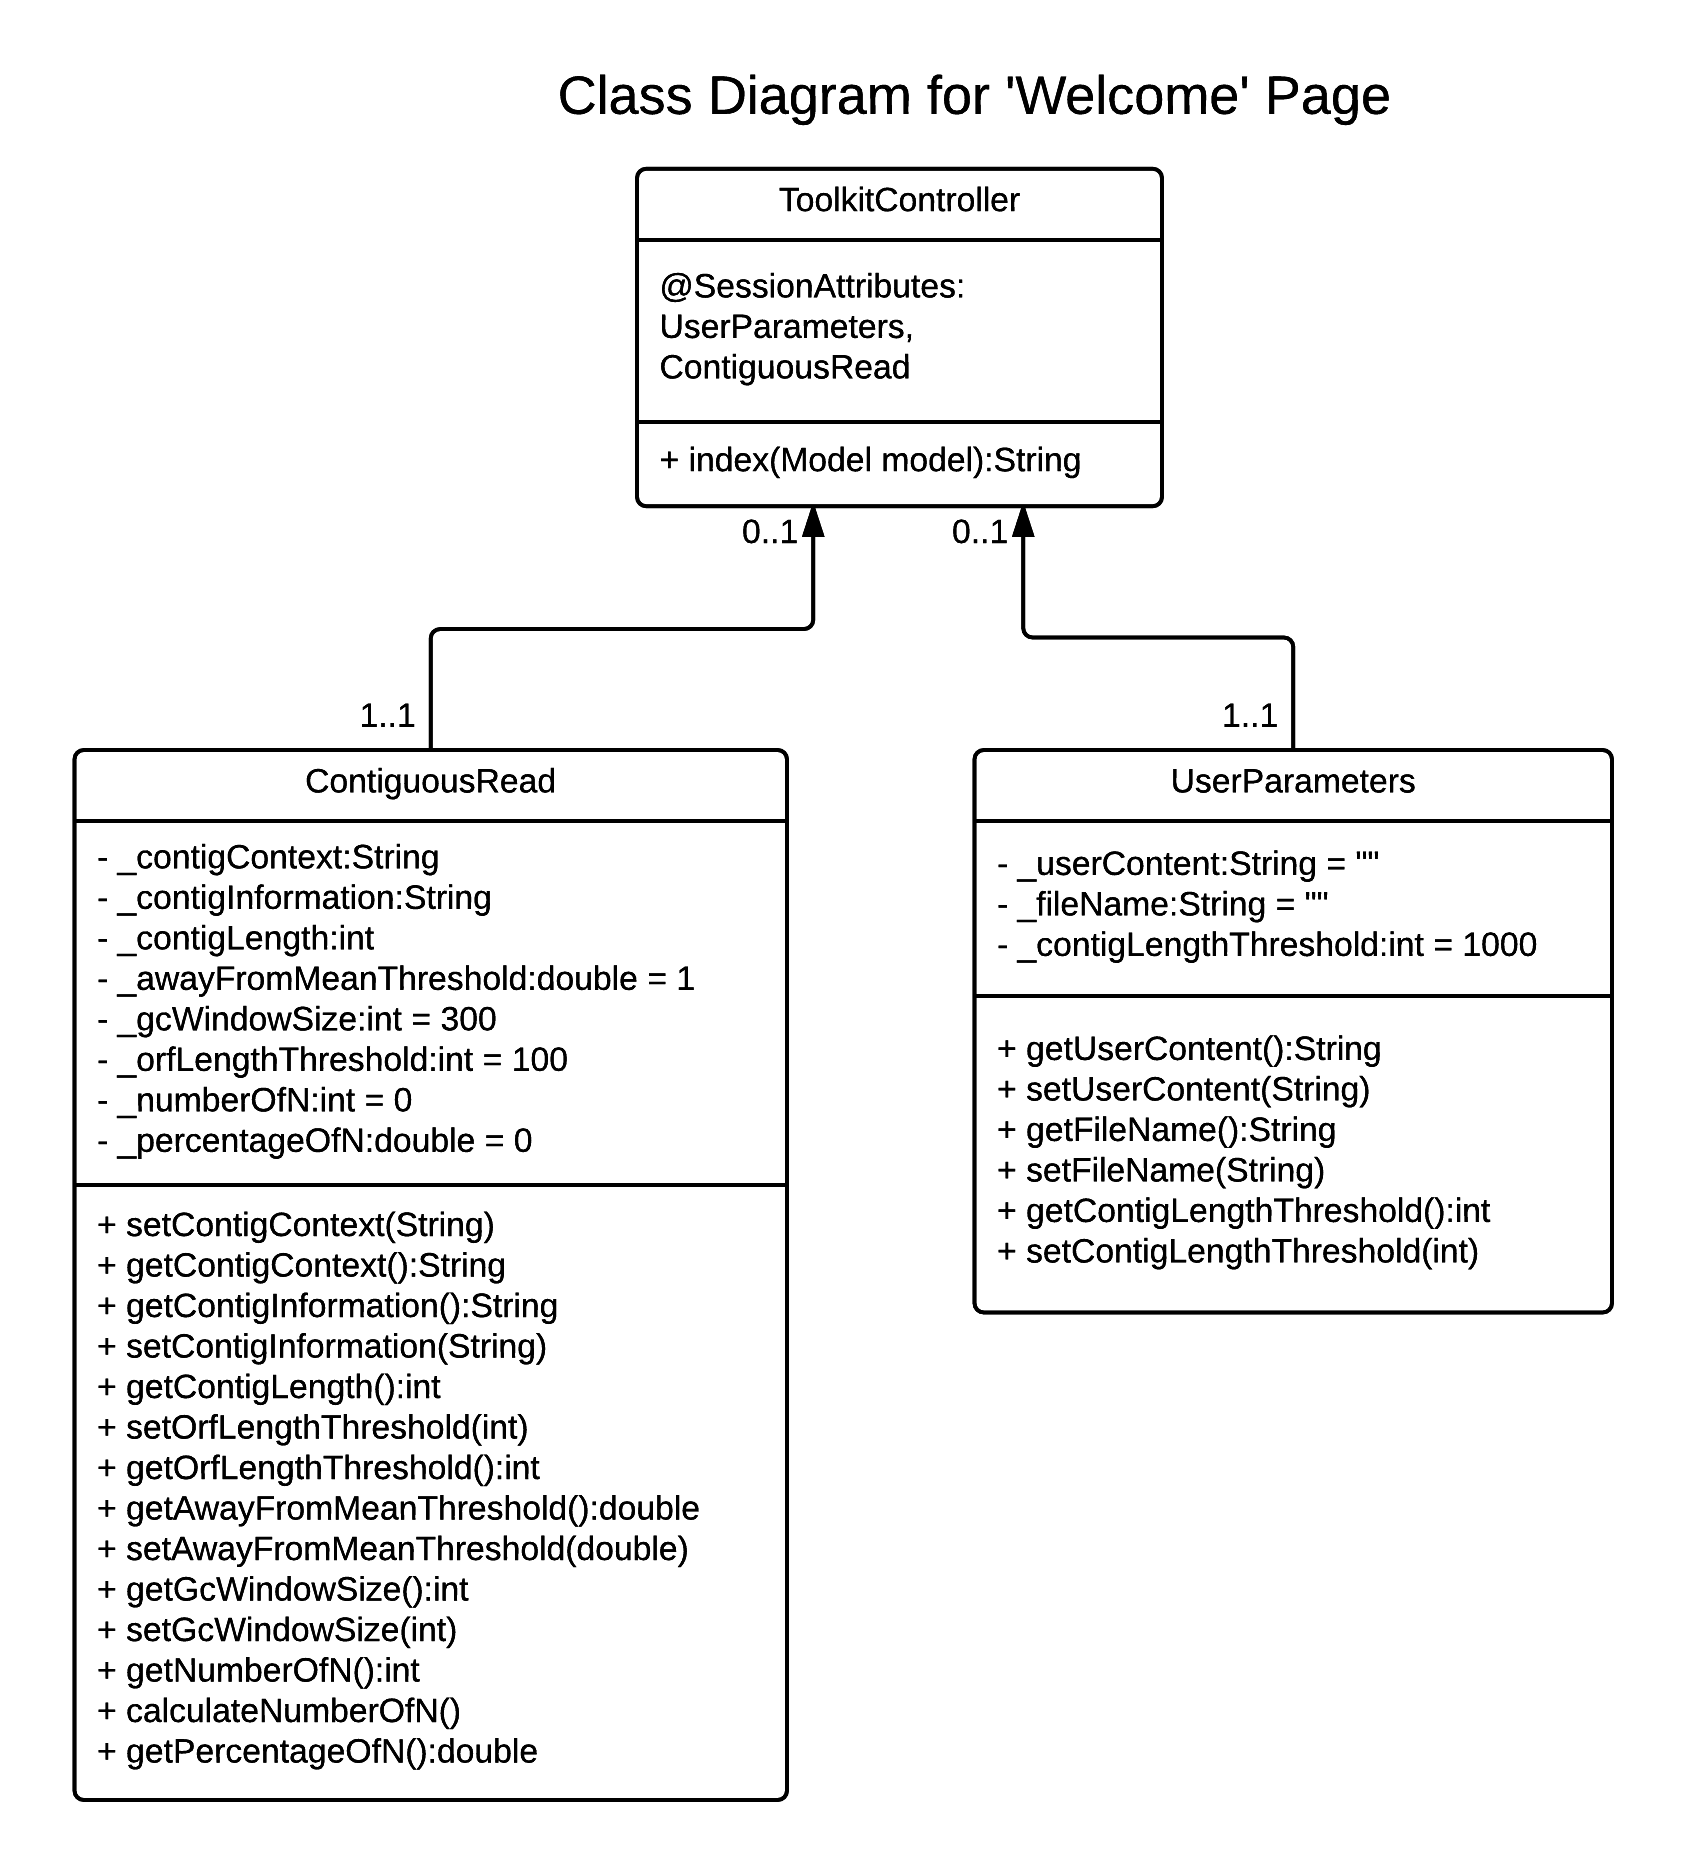
\includegraphics[width=0.7\textwidth]{images/umlwelcomepage}
\caption{Class diagram for the `Welcome Page', and what classes are used upon a Request for the page.}
\end{figure}

\begin{figure}[H]
\centering
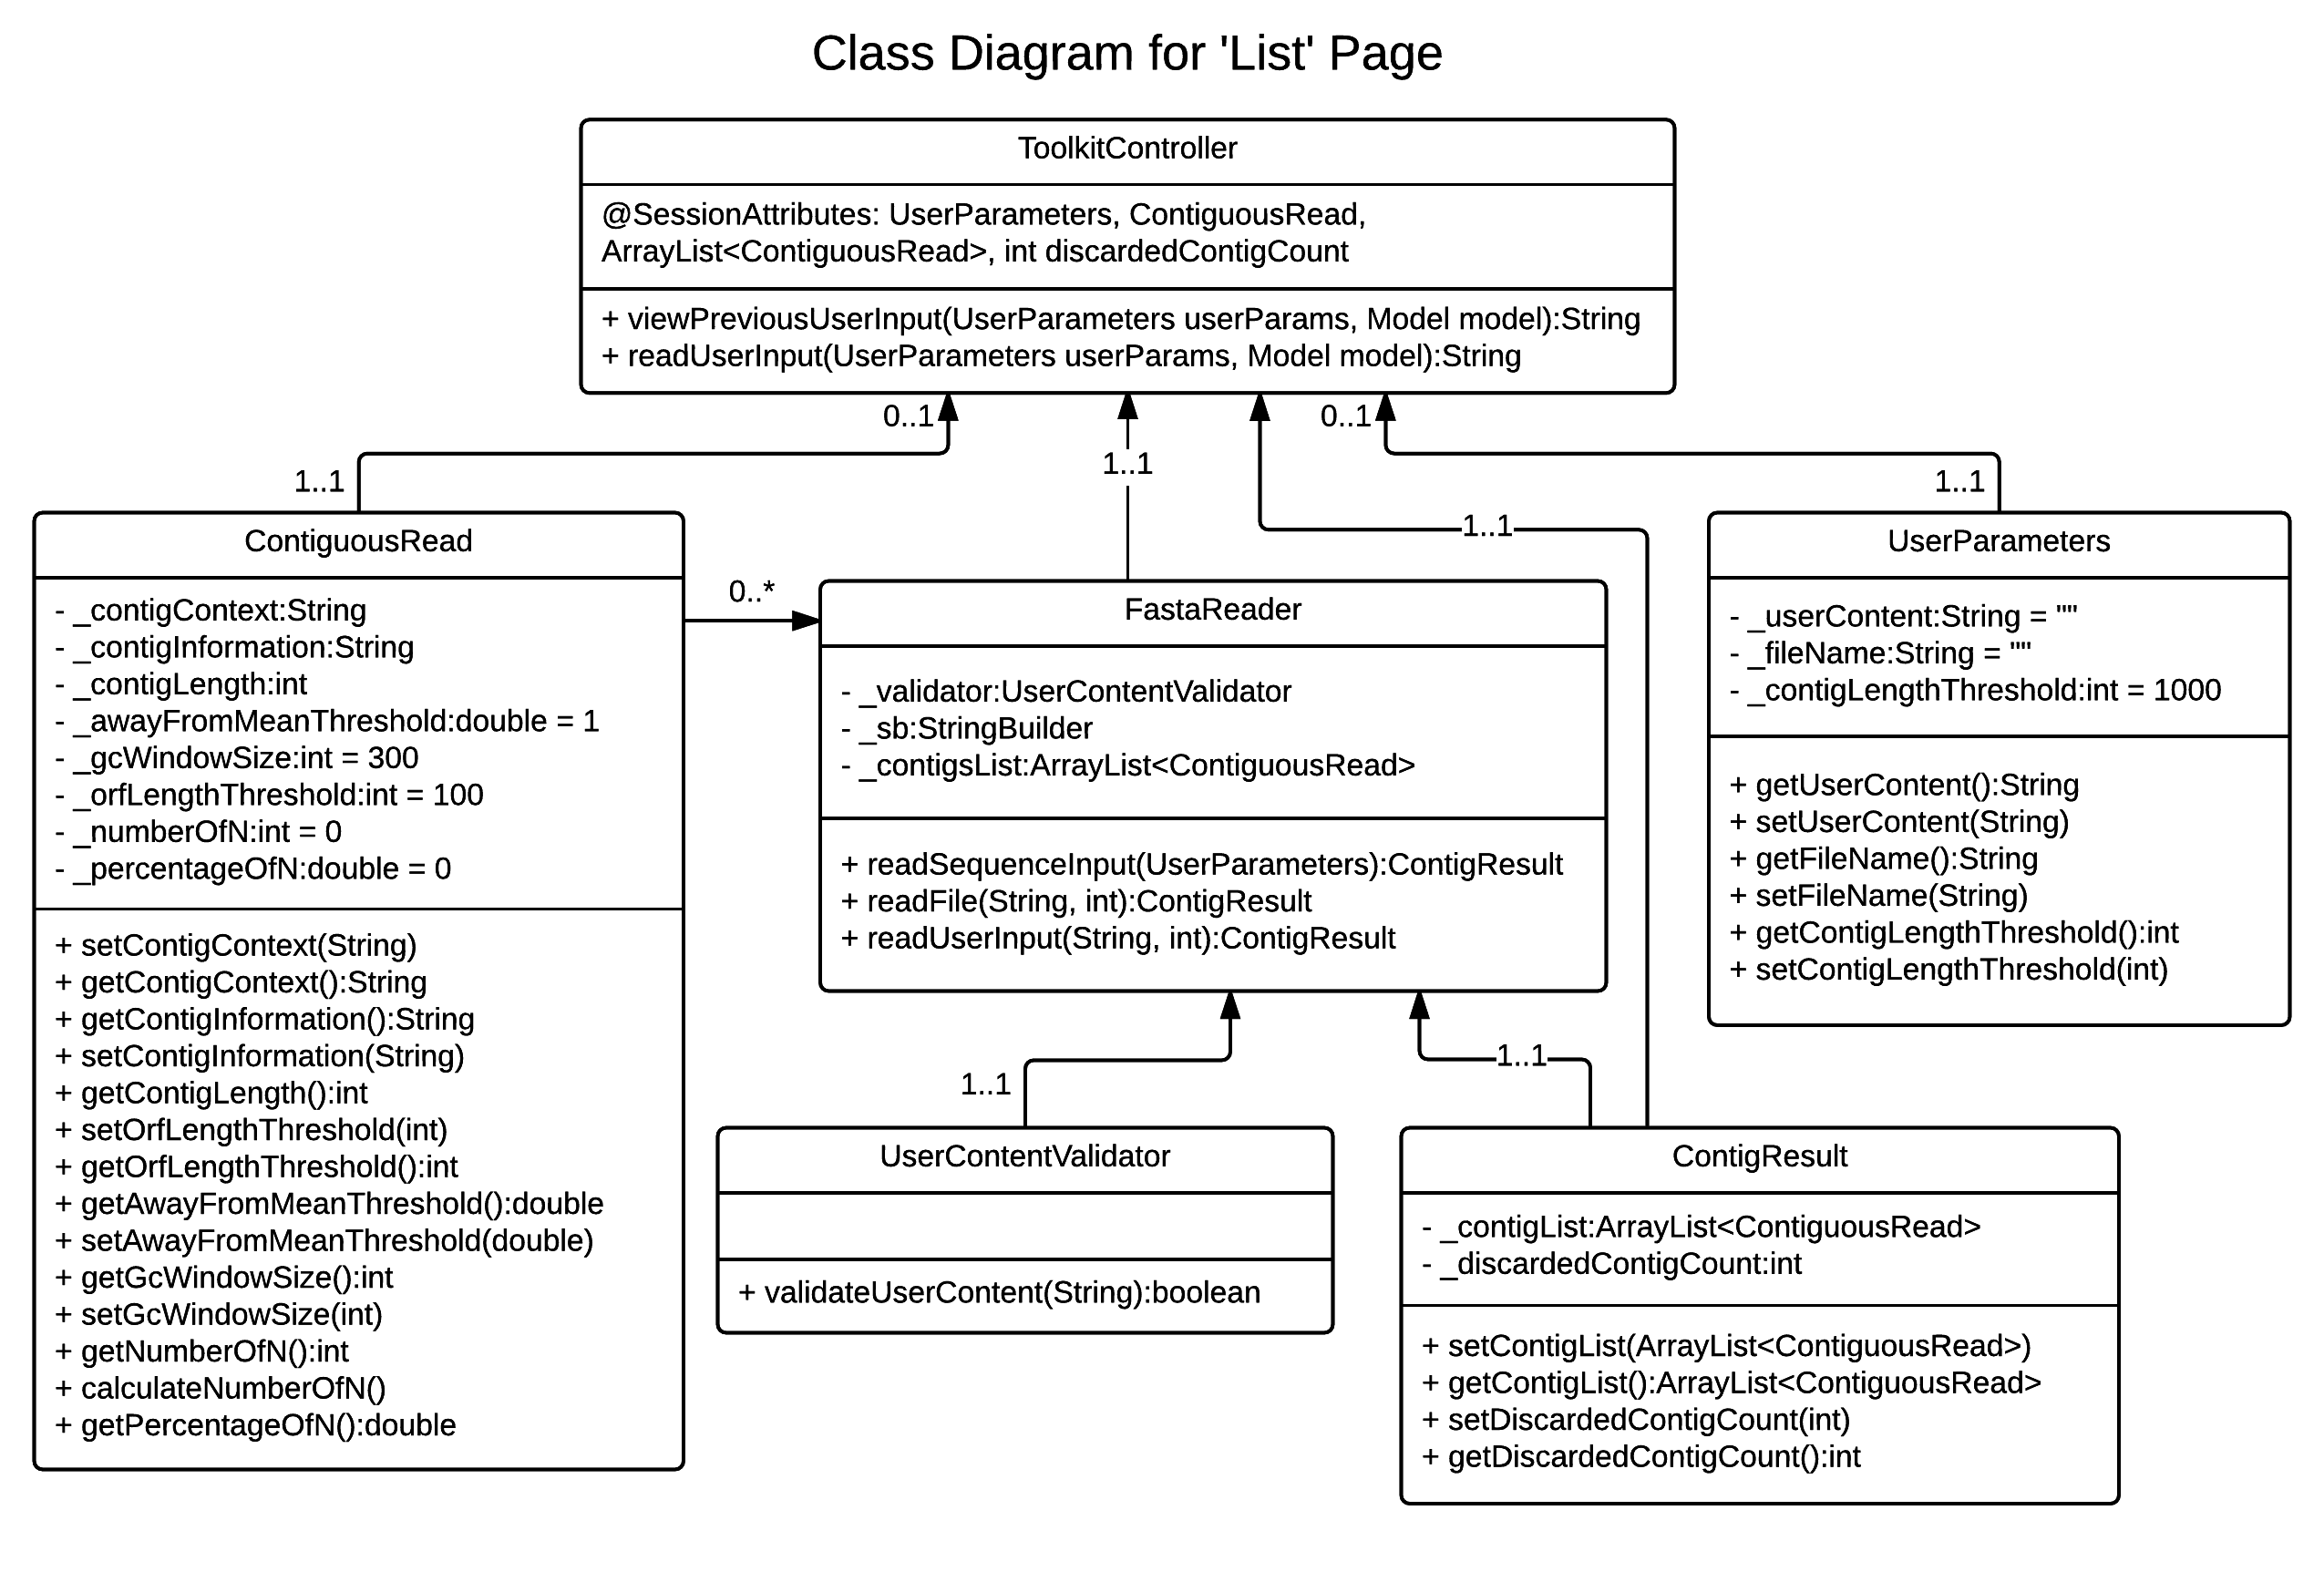
\includegraphics[width=0.8\textwidth]{images/umllistpage}
\caption{Class diagram for the `List Page', and what classes are used upon a Request for the page.}
\end{figure}

\begin{figure}[H]
\centering
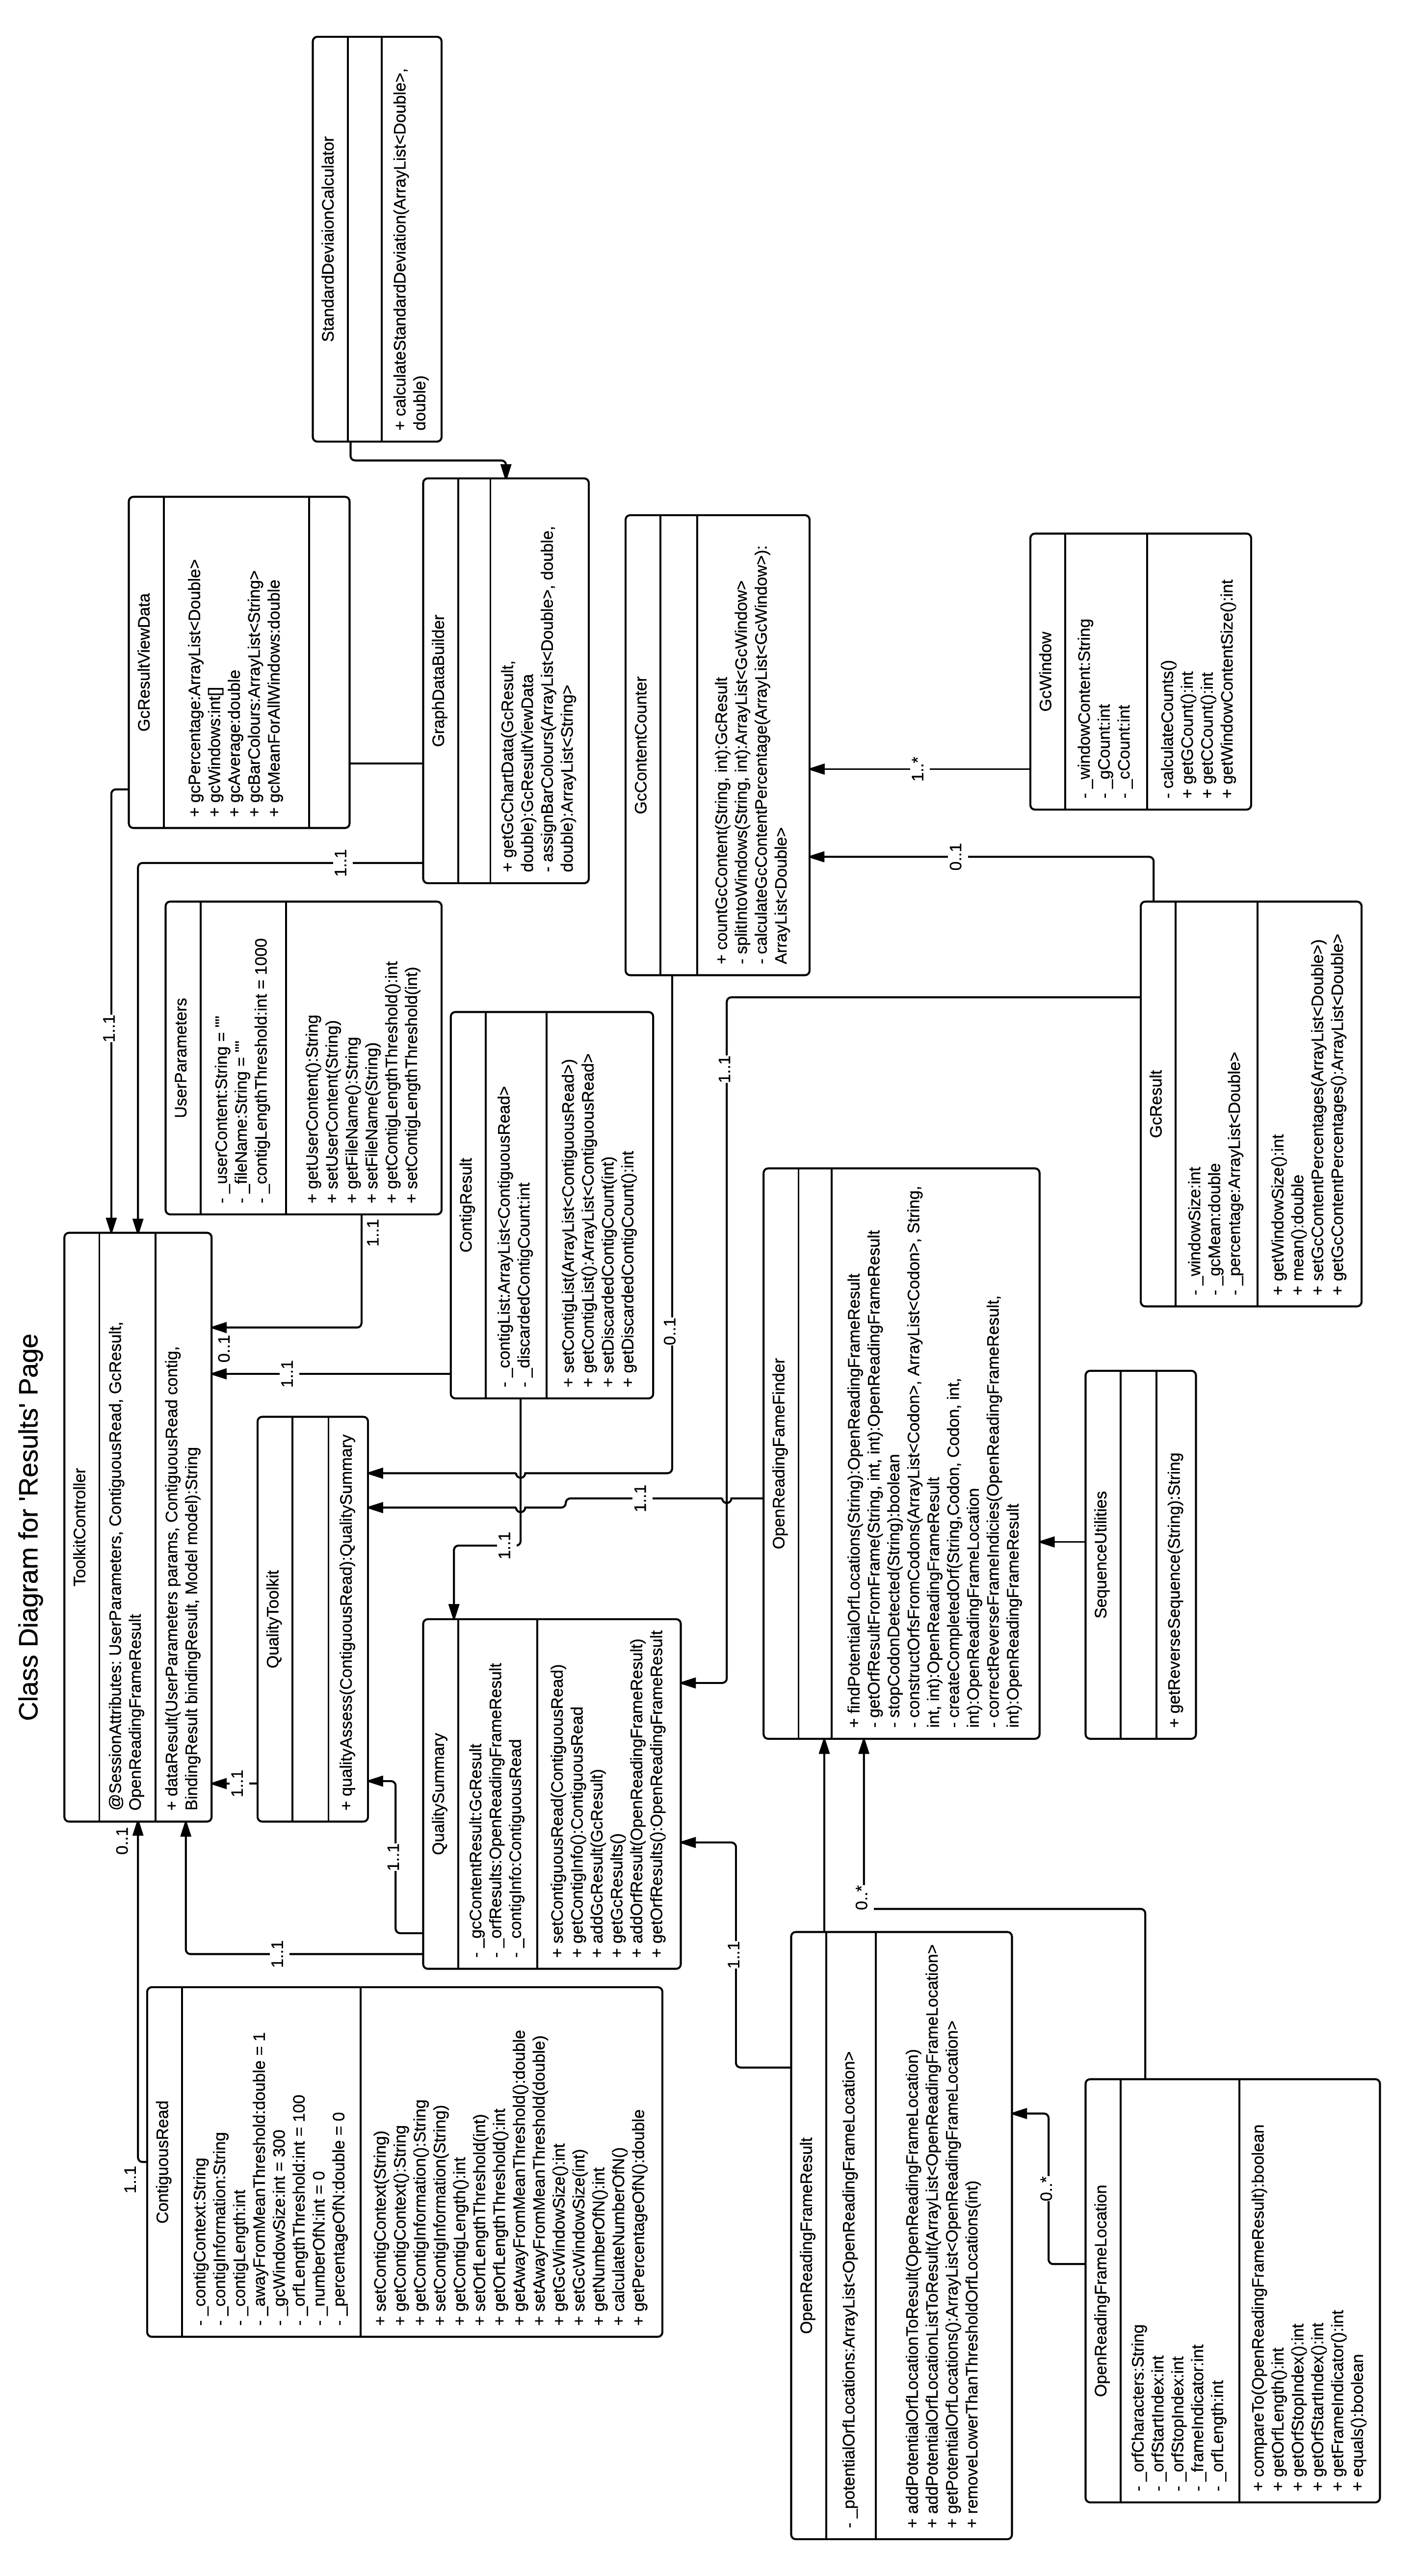
\includegraphics[width=0.8\textwidth]{images/umlresultspageflip}
\caption{Class diagram for the `Results Page', and what classes are used upon a Request for the page.}
\end{figure}

The structure evolved over time due to the nature of XP and using an agile methodology. Even so, the result was that there was a logical sense to the structure of classes, methods belong in the class they live in, some utility classes exist for carrying out operations that don't necessarily need to be within a class that needs that utility and this also left the code easier to maintain and separated. By using utility classes and methods, they can be called by other classes in the future, and the class that uses them doesn't need to know about the implementation internals of the methods they use, only the results.

\subsubsection{View}
The View of the application is where the GUI is presented to the user to be seen in their browser. Designing the application to use the browser was chosen to allow anyone to be able to use the application as long as they are using a modern browser. It is using HTML, HTML5 Canvas and JavaScript, dynamically built using Thymeleaf templates. If any of the template does not process or there is an issue with the users data they are presented with an error page and told to return to the menu and try their task again.

The data for the View comes from the Model, passed by the Controller. In line with keeping responsibilities separated, the Model does not care about how the View displays the data, and the View does not care about the content of the Model data it is passed as long as the data types it expects are present in the Model from the Controller. For example, the ORF Location data is sent to the View as an OpenReadingFrameResult Object, that has a list of OpenReadingFrameLocations and other data about the process. It is then the responsibility of the View to use this data in displaying it in HTML5 Canvas with JavaScript. No additional processing or modifications are carried out on the data at this point, the View just picks up the data and places it on the Canvas element where it expects it should go, based on the content of the data, e.g. an OpenReadingFrameLocation with the `frameIndicator' set as 0 would indicate to the View that it should be placed on Frame 1.

This type of responsibility separation is consistent throughout the application, with one except. There is a GcResultDataView, that is the GcResult data processed into an easy to handle class. This is to make the process for the View far faster than having to get the View to carry out some processing to determine the GcWindows that are out of the mean threshold and additional results to display on the bar chart for the GcResult. While it would be possible to alter the application in order to leave this up to the View, I felt that it would be better to instead serve the View with the window data it needed to put on the chart and the colour codes for each of those window data bars.

\subsubsection{Controller}
The Controller serves as the master for how data flows through the application, making calls to methods from the Model to process the users data, receiving requests from the user via the View and HTML Requests and handling what data is for use in the View. The user may send HTML Requests to the different pages of the application and will receive a response based on the `@RequestMappings' of the Controller. 

For example, a GET on the `list' page will return a page expecting the user to have already submitted some data that has been turned into a list of contigs. A POST on the `list' page however will be expecting that this is a new set of data and process the data submitted into a list of contigs and put them into the users session attributes.

Through every page, a user carries a Session with them and particular session attributes are expected at certain points in @SessionAttributes. For example, a user must have UserParameters and a ContiguousRead in their session parameters in order to be able to view the List and Results page. If they have not visited the Welcome page and submitted data, however, it is not possible for them to have these attributes, and so they are locked out of those pages. This is good behavior as the user should not be able to try and view results for data they have not submitted.

\subsection{Naming Conventions}
I followed a naming convention of attempting to name classes, methods, fields and variables in such a way that a reader could understand what the function of that particular thing was just from the name alone. Private field names all begin with an underscore, e.g. `\_privateField' and everything is written in camel case, starting with a lowercase character, e.g. `thisWouldBeAMethodName()'.

\subsection{User Input}
Based on the background reading, the decided file format to accept was FASTA format. The design allows for user uploading and user pasting of files in the Model methods. However, in the end I decided to keep the design just to handling pasting of data. This was based on a time constraint and issues with file upload limits, security and the need to test. While the functionality has been left in the code, it has been left as a `if I were to continue' functionality to be expanded upon if I had more time to work on file uploading as a priority over different techniques for the quality assessment.

User data is also not kept by the application, it is stored in a user session that expires once they leave the page. This is handled by Java Spring, and set as one of the @SessionAttributes. If the user does not have their session variables, they are presented with the Error page, so they cannot try and access areas of the application/web service where they currently do not have access or the data to do so. This means that the data they have is their own, and not retained by the application or possible for other users to access.

\subsection{Directory Structure}
The directory of the applications structure was designed such that it would reflect the MVC aspect of the application, and make finding resources and particular Classes easier for a reader. The design makes the application easier to maintain in the future and is another way of helping to enforce separation of responsibilities between classes and resource types. In the figure below you can see the way that the directory structure is designed to back this up.

\begin{figure}[H]
\centering
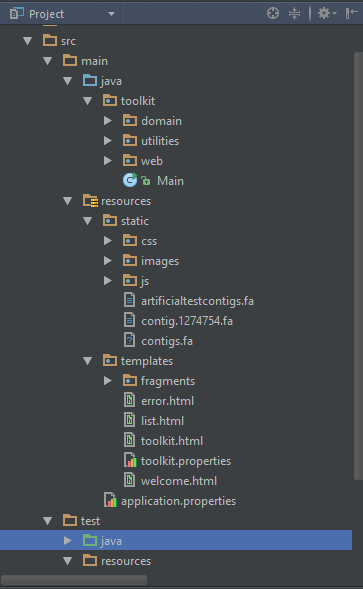
\includegraphics[width=0.5\textwidth]{images/directorystructure}
\caption{The layout of the directory structure for the application.}
\end{figure}

Within the `src/java' folder, there are the sub folders `domain', `utilities' and `web'. Separating the classes out this way helps with the previously mentioned separation of responsibilities. Domain contains the classes for the domain objects themselves and the data and processing (the Model, so GcResult, OpenReadingFrameLocation, etc), Utilities contains utility classes for use by any of the other classes and to allow their functionality to be independent of any domain class and Web contains the Controller classes (ToolkitController, ErrorController).

\subsection{QualitySummary and Results}
In the application, the quality assessment results are returned in a QualitySummary object. This QualitySummary contains references to GcResult and OpenReadingFrameResult. The is the option to have these two implement an interface that might be called QualityResults, and have just an array of QualityResults. This would allow us to add any type of result without needing to know what is in there. However, I chose not to do this as considering the way in which we serve data to the View it seemed okay to be able to have the View called results from the model directly, and through XP developing this any further would go against YAGNI. 

I am aware that in the future if we allowed a user to select what type of processing they wish to use and as more techniques for quality assement are added, this technique would be very useful to implement. It would be possible to do this and in the View have it check for the existence of the expected results, or check if they were empty/null, and then only dynamically include fragments of results that are present. 

\section{User Interface}
Framework mock ups of the user interface. Logo for kicks.

- Input form, why is it this way?
- List - Displaying each contig, why, framework, drop downs
- Paramters - Why did I pick these Paramters, what use are these for the user? Why GC content windows and what size is reasonable? Can demonstrate domain knowledge about the choice of parameters. Up to the user, allowing them to put in stupid numbers, but their results are their own.
- GC Chart - Why does it look like this - Choice of standard deviation and mean, why? What use does this actually have  in showing the user error areas? What about just visually seeing the data? Show the screenshots of areas out of GC content threshold, show the areas where obvious chimera (50/50 example)
- ORF Location - Why did I develop it to look like this? Representing each of the 6 frames, demonstrate the reverse frames are displayed in the correct direction. How did I achieve this and why display it this way and the inner detail? Other approaches? What about the NCBIs version? Ability to click. Also the list? Why have both? They're both useful to have, as a user may want to look at the shortest ORF Location but not be sure where it is even when they read what frame it is. Likewise they may want to see where an ORF Location lies in the list organized into longest to shortest. Why organized into length. Useful to the user to get an idea to further inspect. Why 6 different canvases for the frames? Easier to modify and display on the page.
- Superframe - What is it and why did I consider it. Showing overlaps and where the Red areas may be areas of errors and what to look for. The explanation of it, why explain it this way? 

\section{Support Tools}
For writing the code, I used JetBrains IntelliJ IDE (screenshot of IDE window with some code). This included writing all the code, Java, HTML, CSS, Javascript, ThymeLeaf and any additional properties for setting up Spring Boot. Useful for text highlighting, debugging the code, and tied into my version control, using Git and hosted on GitHub. (screenshot of commits)
\subsection{Version Control}
Using version control to keep a repository of code in case of lost data in event of hardware crash or software corruption. GitHub decent choice, already had a repository on there and Git supported in IntelliJ IDE. In addition, every time I check in, I used continuous integration with CodeShip, allowing me to receive e-mails any time I made a commit to my repo that didn't pass the tests written. Very helpful in discovering issues with failing builds when checking in a change and forgetting to update tests or breaking previously written code as the design changed (show screenshot of failing/passing builds from CodeShip).